\documentclass{beamer}
%\documentclass[handout]{beamer}
\usetheme{Darmstadt}

\usepackage[utf8]{inputenc}
\usepackage{default}
\usepackage{hyperref}
\hypersetup{colorlinks=true,linkcolor=orange,urlcolor=orange}
\usepackage{tikz}

\newcommand{\tango}{\textsc{Tango}}
\newcommand{\corba}{\textsc{Corba}}
\newcommand{\onmiORB}{\textsc{omniORB}}
\newcommand{\zmq}{\textsc{$\varnothing$mq}}
\newcommand{\mysql}{\textsc{MySQL}}
\newcommand{\sardana}{\textsc{Sardana}}
\newcommand{\mambo}{\textsc{Mambo}}
\newcommand{\atk}{\textsc{Atk}}
\newcommand{\taurus}{\textsc{Taurus}}

\newcommand{\todo}[1]{\texttt{\color{red}TODO:} ``\emph{#1}''}

\title[Securing \tango\, Control System]{Securing \tango\, Control System:\\ A brain storming}
\author[Sergi Blanch-Torn\'e]{Sergi Blanch i Torn\'e}
\institute[Universidad de Lleida]{Cryptography \& Graphs\\Math Department\\ Universitat de Lleida}
\date{September 24th, 2013}Se\begin{document}

%------------------------------------ Frame 0.1 ------------------------------%
%\frame{\titlepage}
\begin{frame}
  \titlepage
\end{frame}
%-----------------------------------------------------------------------------%

%------------------------------------ Frame 0.2 ------------------------------%
\begin{frame}
\frametitle{Outline}
\tableofcontents[hideallsubsections]
\end{frame}
%-----------------------------------------------------------------------------%

%%%%%%%%%%%%%%%%%%%%%%%%%%%%%%%%%%%%%%%%%%%%%%%%%%%%%%%%%%%%%%%%%%%%%%%%%%%%%%%
\section{Introduction}

\subsection{Definitions}

%------------------------------------ Frame 1.1 ------------------------------%
\begin{frame}
\frametitle{What is an Industrial Control System? (ICS)}
    \begin{block}{\href{http://en.wikipedia.org/wiki/Industrial_Control_System}{Wikipedia's definition (en)}}
        ``It is a general term that encompasses several types of control systems used in industrial production, including \emph{supervisory control and data acquisition} (\alert<2->{SCADA}) systems, \emph{distributed control systems} (\alert<4->{DCS}), and other smaller control system configurations such as \emph{programmable logic controllers} (\alert<3->{PLC}) often found in the industrial sectors and critical infrastructures.''
    \end{block}
\end{frame}
%-----------------------------------------------------------------------------%

%------------------------------------ Frame 1.2 ------------------------------%
\begin{frame}
    \begin{exampleblock}{What is a Programmable Logic Controllers}
        \begin{figure}[h]
            \centering{
            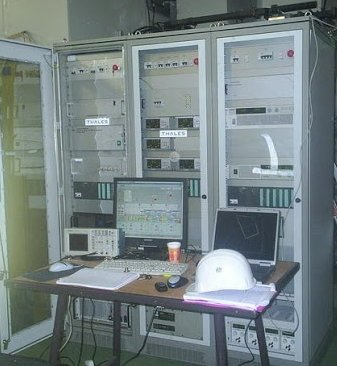
\includegraphics[width=0.5\textwidth]{imgs/ltb_20080527_09-42_006_cut.jpg}
            \caption{Part of a PLC controlled system} \label{fig:linacsPLCs}}
        \end{figure}
    \end{exampleblock}
\end{frame}
%-----------------------------------------------------------------------------%

%------------------------------------ Frame 1.3 ------------------------------%
\begin{frame}
\frametitle{What is an SCADA?}
    \begin{block}{\href{http://es.wikipedia.org/wiki/SCADA}{Wikipedia's definition (es)}}
        ``\emph{Supervisory Control And Data Acquisition} it is a computer software to control and supervise industrial process remotely.''
    \end{block}
    \begin{exampleblock}{Examples of an SCADAs}
        \begin{figure}[h]
            \centering{
            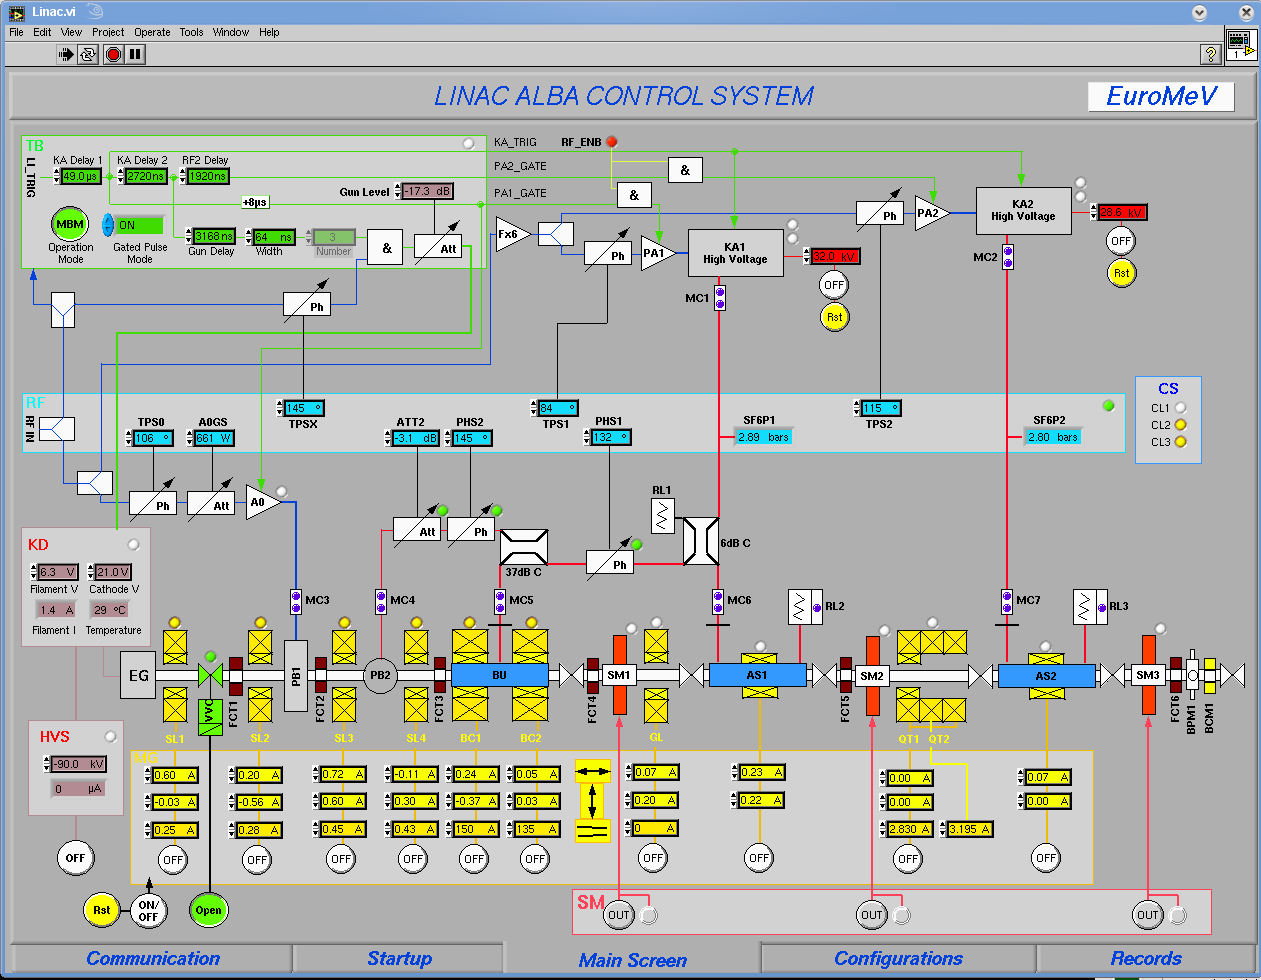
\includegraphics[width=0.4\textwidth]{imgs/labview_tab3_mainScreen.png}
            \caption{Labview as SCADA example} \label{fig:labviewScada}}
        \end{figure}
    \end{exampleblock}
\end{frame}
%-----------------------------------------------------------------------------%

%------------------------------------ Frame 1.4 ------------------------------%
\begin{frame}
\frametitle{What is an Distributed Control System?}
    \begin{block}{\href{http://en.wikipedia.org/wiki/Distributed_control_system}{Wikipedia's definition (en)}}
        a \emph{Distributed Control System} is the computer software for a manufacturing system, process or any kind of dynamic system, in which the controller elements are not central in location (like the brain) but are distributed throughout the system with each component sub-system controlled by one or more controllers.
    \end{block}
    \begin{block}{What is a distributed system?}
        Tanenbaum say \cite{TanenbaumDistr}: \emph{A distributed system is a collection of independent computers that appears to its users as a single coherent system.}
    \end{block}
\end{frame}
%-----------------------------------------------------------------------------%

%------------------------------------ Frame 1.5 ------------------------------%
\begin{frame}
\frametitle{What is a \tango? (I)}
    Tango is an object oriented \emph{Distributed Control System}\\with active collaborative development from:
    \begin{figure}[h]
        \centering{
        
\includegraphics[width=0.7\textwidth]{imgs/tango/00_logos_tango_consortium_members.jpg}
        \caption{Logos of the Tango Consortium Members} \label{fig:tangoConsortium}}
    \end{figure}
\end{frame}
%-----------------------------------------------------------------------------%

%------------------------------------ Frame 1.6 ------------------------------%
\begin{frame}
\frametitle{What is a \tango? (II)}
    \begin{block}{It's an Distributed Control System}
        using \corba\, as a Middleware (\onmiORB),\\ with \zmq\, in the event broadcasting.
    \end{block}
    \begin{block}{What means middleware?}
        Tanenbaum say \cite{TanenbaumDistr}: \emph{It is what supports heterogeneous computers and networks while offering a single system view.}
    \end{block}
\end{frame}
%-----------------------------------------------------------------------------%

%------------------------------------ Frame 1.7 ------------------------------%
\begin{frame}
\frametitle{What is a \tango? (iIII)}
    \begin{block}{\tango\, parts}
        \begin{itemize}
            \item \tango\, core $\Rightarrow$ the Middleware
            \item \tango\, Device Servers $\Rightarrow$ the agents in the DCS
        \end{itemize}
    \end{block}
    \begin{exampleblock}{Device servers, device classes, and devices}
        \todo{Draw a nice picture about what those three things are...}
    \end{exampleblock}
    \begin{block}{What has an Agent (a device)}
        %\begin{itemize}
        %    \item Data types: Boolean, [U]Short, [U]Long[64], Double, String
        %    \item Data dimensions: Scalar, Spectrum, Image
        %\end{itemize}
        \todo{commands,attributes and properties}
    \end{block}
\end{frame}
%-----------------------------------------------------------------------------%

%------------------------------------ Frame 1.8 ------------------------------%
\begin{frame}
%     \begin{block}{The sea of Hardware}
%         \todo{Add the nice picture of the sharks in the sea... With agents representation with interactions (communications, phone book, framework, archiving, user access,...}
        \begin{figure}[h]
            \centering{
                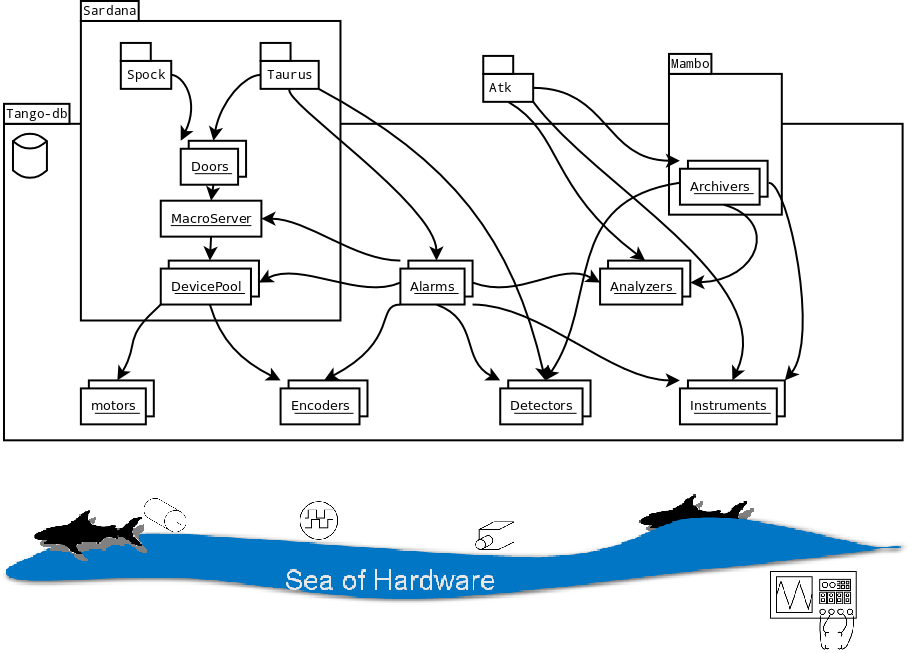
\includegraphics[width=0.75\textwidth]{imgs/tango/tango_layout.png}
                \caption{Tango schematic layout} \label{fig:tangoLayout}
            }
        \end{figure}
%     \end{block}
% communications:
% - synchronous/asynchronous => \onmiORB
% - events => \zmq
% persistent data and phone book of the distributed system
% - tango-db => \mysql
% Framework:
% - \sardana
% Archiving:
% - Mambo
% User access:
% - \atk
% - \taurus
\end{frame}
%-----------------------------------------------------------------------------%

%%%%%%%%%%%%%%%%%%%%%%%%%%%%%%%%%%%%%%%%%%%%%%%%%%%%%%%%%%%%%%%%%%%%%%%%%%%%%%%
\section{Identify scenarios}

\subsection{Use cases of \tango}

%------------------------------------ Frame 1.9 ------------------------------%
\begin{frame}
\frametitle{Optics Lab: Long Term Profiler}
    \begin{figure}[h]
        \centering{
        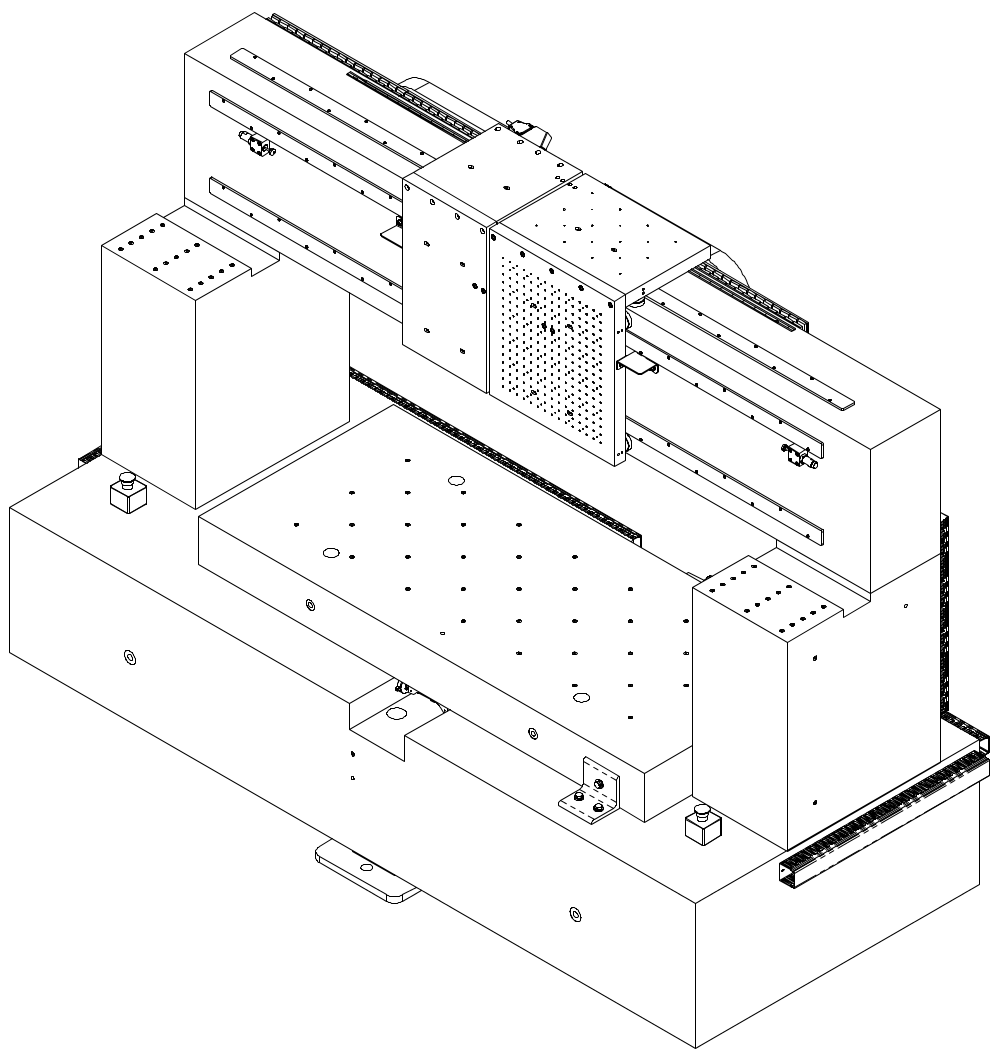
\includegraphics[width=0.65\textwidth]{imgs/laop_ltp_isometric_view.png}
        \caption{drawing of the optics lab LTP} \label{fig:laopLTP}}
    \end{figure}
\end{frame}
%-----------------------------------------------------------------------------%

%------------------------------------ Frame 1.10 -----------------------------%
\begin{frame}
\frametitle{A beamline}
    \begin{center}
         \begin{tikzpicture}
             \node (bl11) at (0,0) {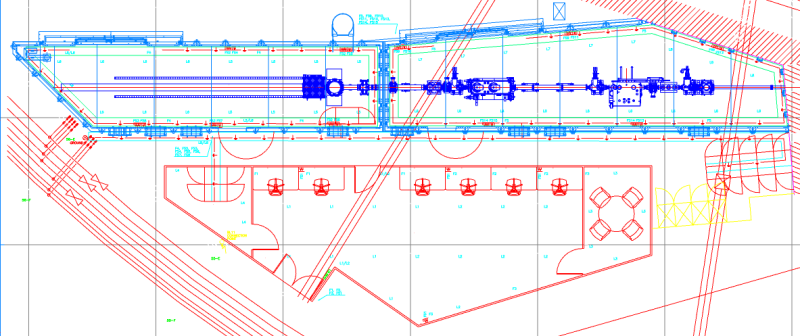
\includegraphics[width=0.75\textwidth]{imgs/2009_bl11_ncd.png}};
             \pause
             \node (ctbl09) at (bl11.south east) {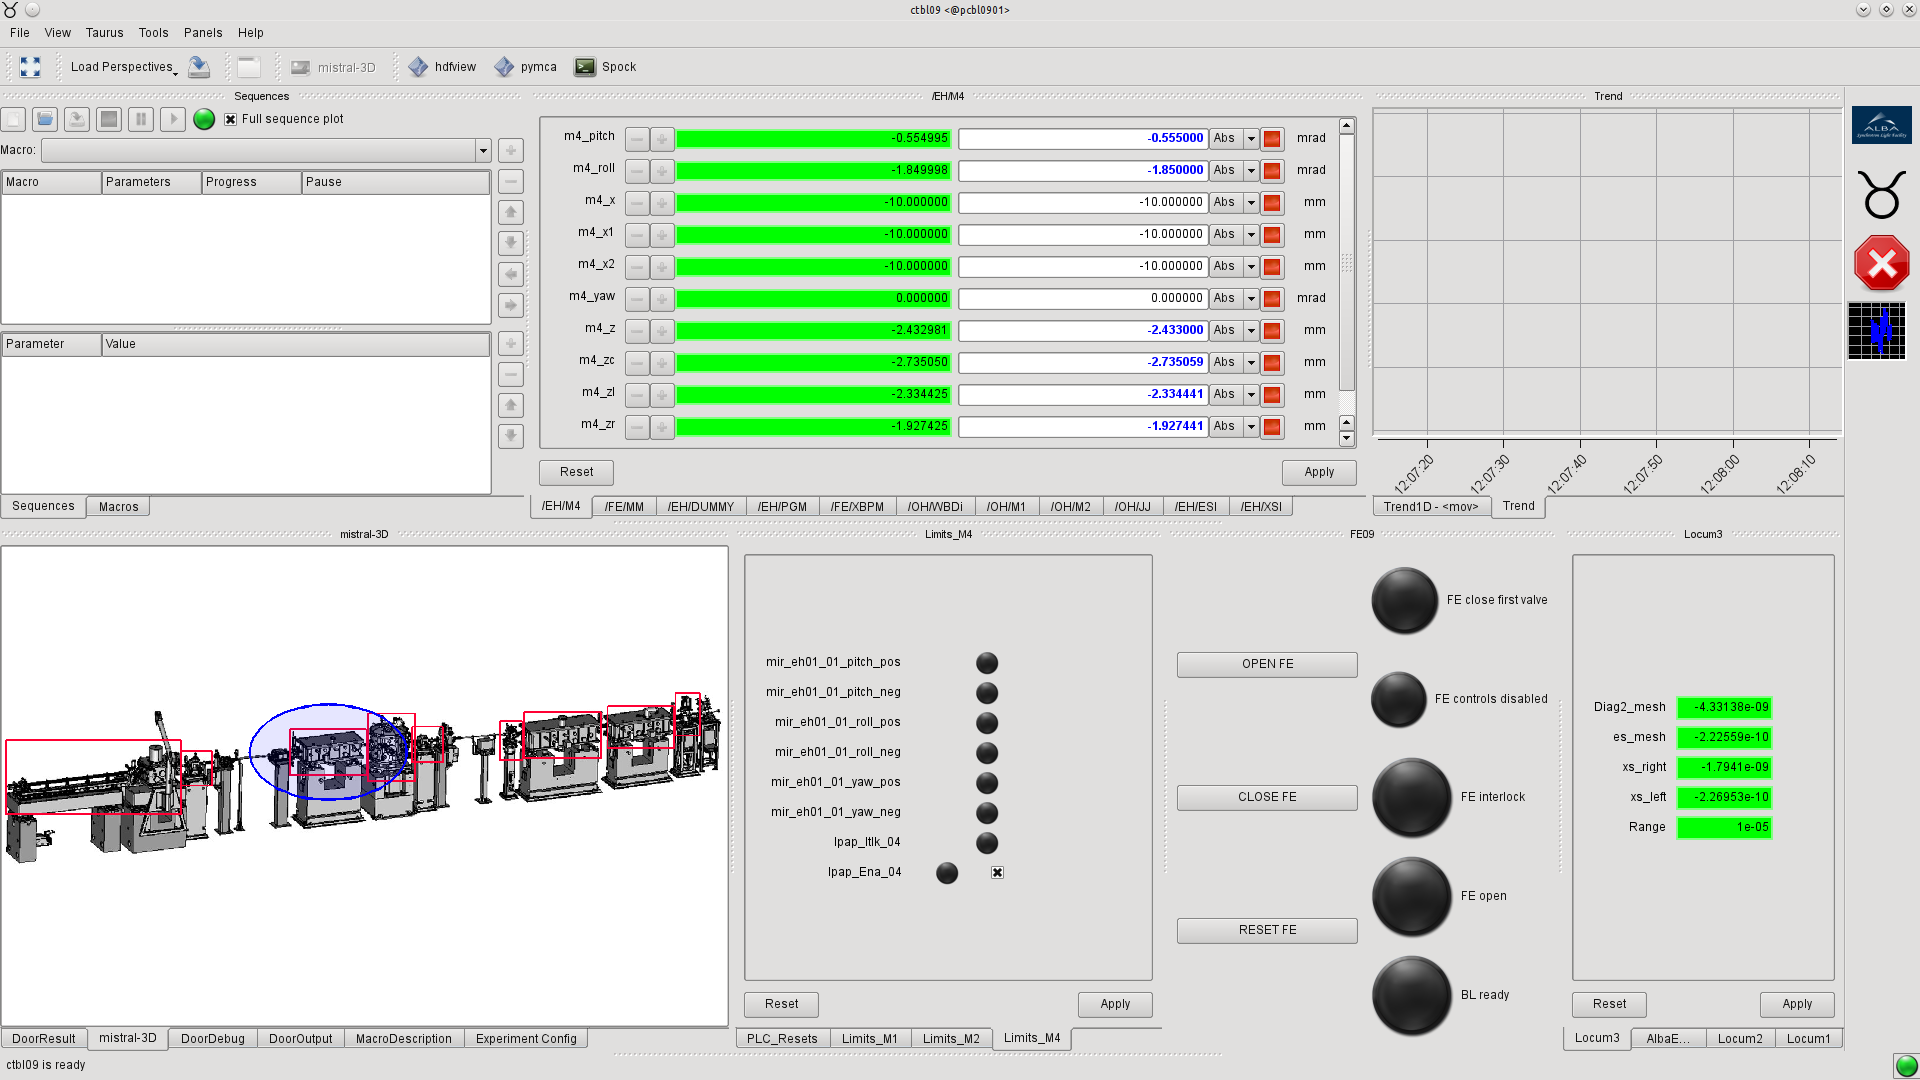
\includegraphics[width=0.75\textwidth]{imgs/20130917_ctbl09.png}};
         \end{tikzpicture}
    \end{center}
\end{frame}
%-----------------------------------------------------------------------------%

%------------------------------------ Frame 1.11 -----------------------------%
\begin{frame}
\frametitle{Control a synchrotron accelerator}
     \begin{itemize}
         \item \todo{Draws of the synchrotron layout and data from the ccdb about the service area numbers}
         \item \todo{List subsystems in the accelerator}
         \begin{itemize}
              \item Timming (132 agents)
              \item Vaccum (1085 agents)
              \item Power supplies (491 agents)
              \item Radio frequency (124 agents)
              \item Diagnostics (744 agents)
              \item<1-|alert@1> +2500 agents
         \end{itemize}
         \item \todo{Astor}
     \end{itemize}
\end{frame}
%-----------------------------------------------------------------------------%

\subsection{In distributed system}

%------------------------------------ Frame 2.1 ------------------------------%
\begin{frame}
\frametitle{Against the transparencies}
    \resizebox{\textwidth}{!}{
        \begin{tabular}{|l|l|}
            \hline
            Access & Hide differences in data representation and how a resource is accessed \\ \hline
            Location & Hide where a resource is located \\ \hline
            Migration & Hide that a resource may move to another location \\ \hline
            Relocation & Hide that a resource may be moved to another location while in use \\ \hline
            Replication & Hide that a resource is replicated \\ \hline
            Concurrency & Hide that a resource may be shared by several competitive users \\ \hline
            Failure & Hide a faulure and recovery of a resource \\ \hline
            Persistence & Hide whether a (software) resource is in memory or on disk \\ \hline
        \end{tabular}
    }
    \begin{block}{Security threads}<2->
        All those transparencies shows at least on security issue
    \end{block}

\end{frame}
%-----------------------------------------------------------------------------%

% %------------------------------------ Frame 2.2 ------------------------------%
% \begin{frame}
% \frametitle{Against the layers}
%     \begin{figure}[h]
%         \centering{
%         %\resizebox{0.5\textwidth}{!}{% PSTricks TeX macro
% Title: /home/serguei/src/Papers/Ensuring_Tango_CtrlSys/imgs/TanenbaumDistributedSystemOrganization.dia
% Creator: Dia v0.97.2
% CreationDate: Sun Aug 11 19:16:03 2013
% For: serguei
% \usepackage{pstricks}
% The following commands are not supported in PSTricks at present
% We define them conditionally, so when they are implemented,
% this pstricks file will use them.
\ifx\setlinejoinmode\undefined
  \newcommand{\setlinejoinmode}[1]{}
\fi
\ifx\setlinecaps\undefined
  \newcommand{\setlinecaps}[1]{}
\fi
% This way define your own fonts mapping (for example with ifthen)
\ifx\setfont\undefined
  \newcommand{\setfont}[2]{}
\fi
\pspicture(3.900000,-19.100000)(24.100000,-5.386312)
\psscalebox{1.000000 -1.000000}{
\newrgbcolor{dialinecolor}{0.000000 0.000000 0.000000}%
\psset{linecolor=dialinecolor}
\newrgbcolor{diafillcolor}{1.000000 1.000000 1.000000}%
\psset{fillcolor=diafillcolor}
\psset{linewidth=0.100000cm}
\psset{linestyle=solid}
\psset{linestyle=solid}
\setlinejoinmode{0}
\newrgbcolor{dialinecolor}{0.000000 0.000000 0.000000}%
\psset{linecolor=dialinecolor}
\pspolygon(4.000000,7.000000)(4.000000,17.000000)(9.690000,17.000000)(9.690000,7.000000)
\psset{linewidth=0.100000cm}
\psset{linestyle=solid}
\psset{linestyle=solid}
\setlinejoinmode{0}
\newrgbcolor{dialinecolor}{0.000000 0.000000 0.000000}%
\psset{linecolor=dialinecolor}
\pspolygon(11.000000,7.000000)(11.000000,17.000000)(16.690000,17.000000)(16.690000,7.000000)
\psset{linewidth=0.100000cm}
\psset{linestyle=solid}
\psset{linestyle=solid}
\setlinejoinmode{0}
\newrgbcolor{dialinecolor}{0.000000 0.000000 0.000000}%
\psset{linecolor=dialinecolor}
\pspolygon(18.000000,7.000000)(18.000000,17.000000)(23.690000,17.000000)(23.690000,7.000000)
\psset{linewidth=0.100000cm}
\psset{linestyle=solid}
\psset{linestyle=solid}
\setlinejoinmode{0}
\newrgbcolor{dialinecolor}{1.000000 1.000000 1.000000}%
\psset{linecolor=dialinecolor}
\pspolygon*(5.000000,11.000000)(5.000000,13.000000)(23.000000,13.000000)(23.000000,11.000000)
\newrgbcolor{dialinecolor}{0.000000 0.000000 0.000000}%
\psset{linecolor=dialinecolor}
\pspolygon(5.000000,11.000000)(5.000000,13.000000)(23.000000,13.000000)(23.000000,11.000000)
\setfont{Helvetica}{0.800000}
\newrgbcolor{dialinecolor}{0.000000 0.000000 0.000000}%
\psset{linecolor=dialinecolor}
\rput(14.000000,12.000000){\psscalebox{1 -1}{Tango Middleware}}
\psset{linewidth=0.100000cm}
\psset{linestyle=solid}
\psset{linestyle=solid}
\setlinejoinmode{0}
\newrgbcolor{dialinecolor}{1.000000 1.000000 1.000000}%
\psset{linecolor=dialinecolor}
\pspolygon*(5.000000,8.000000)(5.000000,10.000000)(23.000000,10.000000)(23.000000,8.000000)
\newrgbcolor{dialinecolor}{0.000000 0.000000 0.000000}%
\psset{linecolor=dialinecolor}
\pspolygon(5.000000,8.000000)(5.000000,10.000000)(23.000000,10.000000)(23.000000,8.000000)
\setfont{Helvetica}{0.800000}
\newrgbcolor{dialinecolor}{0.000000 0.000000 0.000000}%
\psset{linecolor=dialinecolor}
\rput(14.000000,9.000000){\psscalebox{1 -1}{Distributed application}}
\psset{linewidth=0.100000cm}
\psset{linestyle=solid}
\psset{linestyle=solid}
\setlinejoinmode{0}
\newrgbcolor{dialinecolor}{0.000000 0.000000 0.000000}%
\psset{linecolor=dialinecolor}
\pspolygon(5.000000,14.000000)(5.000000,16.000000)(9.000000,16.000000)(9.000000,14.000000)
\setfont{Helvetica}{0.800000}
\newrgbcolor{dialinecolor}{0.000000 0.000000 0.000000}%
\psset{linecolor=dialinecolor}
\rput(7.000000,15.000000){\psscalebox{1 -1}{Local OS}}
\psset{linewidth=0.100000cm}
\psset{linestyle=solid}
\psset{linestyle=solid}
\setlinejoinmode{0}
\newrgbcolor{dialinecolor}{0.000000 0.000000 0.000000}%
\psset{linecolor=dialinecolor}
\pspolygon(12.000000,14.000000)(12.000000,16.000000)(16.000000,16.000000)(16.000000,14.000000)
\setfont{Helvetica}{0.800000}
\newrgbcolor{dialinecolor}{0.000000 0.000000 0.000000}%
\psset{linecolor=dialinecolor}
\rput(14.000000,15.000000){\psscalebox{1 -1}{Local OS}}
\psset{linewidth=0.100000cm}
\psset{linestyle=solid}
\psset{linestyle=solid}
\setlinejoinmode{0}
\newrgbcolor{dialinecolor}{0.000000 0.000000 0.000000}%
\psset{linecolor=dialinecolor}
\pspolygon(19.000000,14.000000)(19.000000,16.000000)(23.000000,16.000000)(23.000000,14.000000)
\setfont{Helvetica}{0.800000}
\newrgbcolor{dialinecolor}{0.000000 0.000000 0.000000}%
\psset{linecolor=dialinecolor}
\rput(21.000000,15.000000){\psscalebox{1 -1}{Local OS}}
\psset{linewidth=0.200000cm}
\psset{linestyle=solid}
\psset{linestyle=solid}
\setlinecaps{0}
\newrgbcolor{dialinecolor}{0.000000 0.000000 0.000000}%
\psset{linecolor=dialinecolor}
\psline(4.000000,19.000000)(24.000000,19.000000)
\psset{linewidth=0.200000cm}
\psset{linestyle=solid}
\psset{linestyle=solid}
\setlinecaps{0}
\newrgbcolor{dialinecolor}{0.000000 0.000000 0.000000}%
\psset{linecolor=dialinecolor}
\psline(7.000000,17.000000)(7.000000,19.000000)
\psset{linewidth=0.200000cm}
\psset{linestyle=solid}
\psset{linestyle=solid}
\setlinecaps{0}
\newrgbcolor{dialinecolor}{0.000000 0.000000 0.000000}%
\psset{linecolor=dialinecolor}
\psline(14.000000,17.000000)(14.000000,19.000000)
\psset{linewidth=0.200000cm}
\psset{linestyle=solid}
\psset{linestyle=solid}
\setlinecaps{0}
\newrgbcolor{dialinecolor}{0.000000 0.000000 0.000000}%
\psset{linecolor=dialinecolor}
\psline(21.000000,17.000000)(21.000000,19.000000)
\setfont{Helvetica}{0.800000}
\newrgbcolor{dialinecolor}{0.000000 0.000000 0.000000}%
\psset{linecolor=dialinecolor}
\rput[l](5.000000,4.000000){\psscalebox{1 -1}{}}
\setfont{Helvetica}{0.800000}
\newrgbcolor{dialinecolor}{0.000000 0.000000 0.000000}%
\psset{linecolor=dialinecolor}
\rput(7.000000,6.000000){\psscalebox{1 -1}{Machine A}}
\setfont{Helvetica}{0.800000}
\newrgbcolor{dialinecolor}{0.000000 0.000000 0.000000}%
\psset{linecolor=dialinecolor}
\rput(7.000000,6.800000){\psscalebox{1 -1}{}}
\setfont{Helvetica}{0.800000}
\newrgbcolor{dialinecolor}{0.000000 0.000000 0.000000}%
\psset{linecolor=dialinecolor}
\rput(14.000000,6.000000){\psscalebox{1 -1}{Machine B}}
\setfont{Helvetica}{0.800000}
\newrgbcolor{dialinecolor}{0.000000 0.000000 0.000000}%
\psset{linecolor=dialinecolor}
\rput(21.000000,6.000000){\psscalebox{1 -1}{Machine C}
\endpspicture}
%         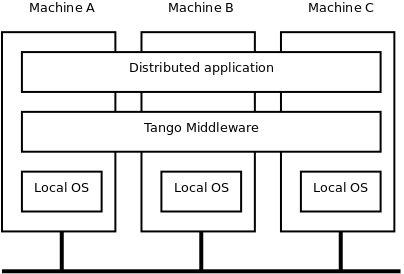
\includegraphics[width=0.5\textwidth]{imgs/TanenbaumDistributedSystemOrganization.png}
%         \caption{From \cite{TanenbaumDistr}, A distributed system organized as middleware} \label{fig:TanenbaumDistributedSystemOrganization}}
%     \end{figure}
% \end{frame}
% %-----------------------------------------------------------------------------%

\subsection{In security engineering}

%------------------------------------ Frame 2.3 ------------------------------%
\begin{frame}
\frametitle{Basics on \emph{information security}}
    \begin{enumerate}
        \item Confidentiality
        \uncover<2->{
            \begin{itemize}
                \item Information must be disclosed only to the authorized.
            \end{itemize}
        }
        \item Integrity
        \uncover<3->{
            \begin{itemize}
                \item Only authorized can set in the system.
            \end{itemize}
        }
        \item Availability
        \uncover<4->{
            \begin{itemize}
                \item Information must be accessible for those who are authorized.
            \end{itemize}
        }
        \item Authenticity
        \uncover<5->{
            \begin{itemize}
                \item Information must only be emitted by the authorized.
            \end{itemize}
        }
        \item Non-repudiation
        \uncover<6->{
            \begin{itemize}
                \item Forbid validity changes on the information emitters.
            \end{itemize}
        }
        %until here they are the bases of information security
        \uncover<8->{
            \item Auditory
            \begin{itemize}
                \item trace who access where\\ (extremely useful for a security breach analysis).
            \end{itemize}
        }
    \end{enumerate}
    \begin{block}{}<7>
        Those first 5 are the basics of the \href{http://en.wikipedia.org/wiki/Information_security}{Information Security}
    \end{block}
\end{frame}

% %-----------------------------------------------------------------------------%

\subsection{Vulnerable attacks}

%------------------------------------ Frame 2.4 ------------------------------%
\begin{frame}
    \begin{block}{Passive}
        \begin{itemize}
            \item Eavesdropping
        \end{itemize}
    \end{block}
    \begin{block}{Active}
        \begin{itemize}
            \item Men-in-the-middle
            \item Spoofing
            \item Noise-Interruption-poisoning: Block transmissions
            \begin{itemize}
                \item Includes [D]DoS
            \end{itemize}
            \item Modification/Fabrication: agent impersonate
        \end{itemize}
    \end{block}
    \begin{block}{counter-measures}
        \begin{itemize}
            \item Intrusion detection and recovery
        \end{itemize}
    \end{block}
\end{frame}
%-----------------------------------------------------------------------------%

%%%%%%%%%%%%%%%%%%%%%%%%%%%%%%%%%%%%%%%%%%%%%%%%%%%%%%%%%%%%%%%%%%%%%%%%%%%%%%%
\section{Cryptography engineering}

\subsection{Security threads}

%------------------------------------ Frame 3.1 ------------------------------%
\begin{frame}
\frametitle{Security threads, policies and mechanisms}
    \begin{itemize}
        \item Thread model:\\From ``Security engineering''\cite{SecEngRossAnderson},\\based on where the thread usually comes from
         \uncover<2->{
            \begin{itemize}
                \item Hospital
                \item Bank
                \item Military base
            \end{itemize}
        }
        \item<3-> References also in ``Cryptography Engineering''\cite{cryptoEngineering}.
        \item<4-> `Practical paranoia' from ``Practical cryptography''\cite{PractCryptoSchneier}:
        \uncover<4->{
            \begin{itemize}
                \item Identify threads
                \item Evaluate attack capabilities
            \end{itemize}
        }
    \end{itemize}
    \begin{alertblock}{}<5->
        Do not left all your security in ISO/IEC 27000-series!
    \end{alertblock}
\end{frame}
%-----------------------------------------------------------------------------%

\subsection{Labelling}

%------------------------------------ Frame 3.2 ------------------------------%
\begin{frame}
\frametitle{Security levels}
    European commission \emph{fiche 17} \\``Exchange of EU classified information'' \cite{fiche17EU}
    \begin{itemize}
        \item Open or Unclassified
        \item Confidential
        \item Secret
        \item Top-Secret
    \end{itemize}
   \begin{exampleblock}{Sub-classifications}<2->
       Elements in a group can have internal subsets. Agents with ``Top-secret'' access only under one subsystem, but ``Confidential'' under another.
   \end{exampleblock}
\end{frame}
%-----------------------------------------------------------------------------%

%%%%%%%%%%%%%%%%%%%%%%%%%%%%%%%%%%%%%%%%%%%%%%%%%%%%%%%%%%%%%%%%%%%%%%%%%%%%%%%
\section{Proposed solutions}

% authentication of agents and users
% encryption of data transmitted:
% - solutions for synchronous/asynchronous
% - solutions for events
% secure the tango-db access: query and write

\subsection{Authentication}

%------------------------------------ Frame 4.1 ------------------------------%
\begin{frame}
\frametitle{Authentication}
    \begin{block}{}
        \begin{itemize}
            \item Agent authentication
            \item User authentication (PAM in Unix)
        \end{itemize}
    \end{block}
    \begin{exampleblock}{}<2->
        In TLS what is authenticated is the server, almost never the client.
    \end{exampleblock}
    \begin{block}{Rights}<3->
         Who have rights to do any read/write action\\
         \emph{Access Control Levels: would be similar than linux permissions}\\
         But multilevel and both directions.
    \end{block}
    \begin{alertblock}{Tools}<4->
        \begin{itemize}
            \item Elliptic curve cryptosystem for TLS (RFC4492 \cite{rfc4492})
            \item This one allow any curve (prime\&char2) in WRF,\\unlike RFC6637 \cite{rfc6637}
        \end{itemize}
    \end{alertblock}
\end{frame}
%-----------------------------------------------------------------------------%

\subsection{Encryption}

%------------------------------------ Frame 4.2 ------------------------------%
\begin{frame}
\frametitle{Encryption}
    \begin{itemize}
        \item Encrypt what has send to an agent
        \item Encrypt what has been answered by an agent
        \item Encrypt events emitted
    \end{itemize}
    \begin{exampleblock}{}<2->
        \begin{itemize}
            \item There are transmissions of single booleans to arrays of tenths of thousands of 64bit elements.
            \item Neither forget the frequency that they can be transmitted.
        \end{itemize}
    \end{exampleblock}
    \begin{alertblock}{Tools}<3->
        \begin{itemize}
            \item Elliptic curves cryptosystem for \emph{key exchange}
            \item (generalized) Rijndael and/or Stream cyphers\\for data transmission and event broadcasting
        \end{itemize}
    \end{alertblock}
\end{frame}
%-----------------------------------------------------------------------------%

\subsection{Database}

%------------------------------------ Frame 4.3 ------------------------------%
\begin{frame}
\frametitle{Database access}
    \begin{itemize}
        \item \tango-db is the ``phone guide'' of the system\\also stores persistent data, like the properties
        \item It is necessary to record over the properties:
        \begin{itemize}
            \item Who and when modifies
            \item Who and when reads (read should be also protectable)
        \end{itemize}
        \item Should be possible to restrict areas of the ``phone book''
        \begin{itemize}
            \item It doesn't have much sense to say where an agent runs if you don't have right to talk with it
            \item this must not replace agent request for authentication of the requester.
        \end{itemize}
    \end{itemize}
    \begin{alertblock}{Tools}<2->
        \begin{itemize}
            \item Homomorphic encryption/Ordered cryptography
        \end{itemize}
    \end{alertblock}
\end{frame}
%-----------------------------------------------------------------------------%

%%%%%%%%%%%%%%%%%%%%%%%%%%%%%%%%%%%%%%%%%%%%%%%%%%%%%%%%%%%%%%%%%%%%%%%%%%%%%%%
\section{Reference Papers}

%\frame{\tableofcontents[currentsection,hideothersubsections]}
\frame{\tableofcontents[sectionstyle=show/hide,subsectionstyle=show/show/hide]}

%------------------------------------ Frame 5.1 ------------------------------%
\begin{frame}
\frametitle{(free) Paper sources}
\begin{itemize}
 \item \href{http://www.iacr.org/}{International Association for Cryptologic Research}\\(e-print \& archiver)
 \item \href{http://arxiv.org(}{arxiv} (open access e-print archiver)
 \item \href{http://vixra.org/}{vixra} (alternative open e-print archiver)
 \item \href{http://citeseerx.ist.psu.edu/}{citeseer} (scientific search engine)
 \item \href{http://scholar.google.com/}{scholar} (Google's indexer)
 \item \href{http://www.informatik.uni-trier.de/~ley/db/}{dblp} (bib reference)
\end{itemize} 
\end{frame}
%-----------------------------------------------------------------------------%

\subsection{Zero-knowledge proof}

%------------------------------------ Frame 5.2 ------------------------------%
\begin{frame}
\frametitle{Zero-knowledge proof for authentication}
    \begin{itemize}
        \item S.Mart\'{\i}nez, ``\emph{Protocolos de seguridad para sistemas de identificaci\'on por radiofrecuencia}''. PhD Thesis UdL, march 2011. Directed by: Concepci\'o Roig and Magda Valls.\cite{Santi11}
        \item BSI TR-03110:``\emph{Advanced security mechanisms for machine readable travel documents.}''.\cite{BSI_TR-03110}
    \end{itemize}
\end{frame}
%-----------------------------------------------------------------------------%

\subsection{Session key exchange}

%------------------------------------ Frame 5.3 ------------------------------%
\begin{frame}
\frametitle{key exchange}
    \begin{itemize}
        \item R. Tom\`as, ``\emph{Volcans d'isogenies de corbes el$\cdot$l\'{\i}ptiques: Aplicacions criptogr\`afiques en targetes intel$\cdot$ligents}''. PhD Thesis UdL, march 2011. Directed by: Josep M. Miret and Daniel Sadornil.\cite{Rosana11}
        \item BSI TR-03111:``\emph{Elliptic curve cryptography, version 2.0}''.\cite{BSI_TR-03111}
        \item S. Blake-Wilson, N. Bolyard, V. Gupta, C. Hawk, and B. Moeller, ``\emph{Elliptic curve cryptography (ecc) cipher suites for transport layer security (tls)}'' May 2006. RFC4492. \cite{rfc4492}

    \end{itemize}
\end{frame}
%-----------------------------------------------------------------------------%

% \subsection{Secret broadcasting}
% 
% %------------------------------------ Frame 5.4 ------------------------------%
% \begin{frame}
% \frametitle{Secret broadcasting}
% \end{frame}
% %-----------------------------------------------------------------------------%

\subsection{Symmetric and stream cyphers}

%------------------------------------ Frame 5.5 ------------------------------%
\begin{frame}
\frametitle{Symmetric cyphers}
    \begin{itemize}
        \item ``\emph{Specification for the advanced encryption standard (aes).}'' Federal Information Processing Standards Publication 197, 2001.\cite{AES-FIPS}
        \item J. Daemen and V. Rijmen, ``\emph{The Design of Rijndael}''. Secaucus, NJ, USA: Springer-Verlag New York, Inc., 2002. \cite{Daemen:2002:DR:560131}
        \item<1-|alert@1> Smaller block size requested
        \item<1-|alert@1> Bigger block size would be better than block cipher modes (CBC, CFB, CTR)
        \item J. Schaad and R. Housley, ``\emph{Advanced Encryption Standard (AES) Key Wrap Algorithm.}'' Sept. 2002. RFC3394 \cite{rfc3394}

    \end{itemize}
\end{frame}
%-----------------------------------------------------------------------------%

%------------------------------------ Frame 5.6 ------------------------------%
\begin{frame}
\frametitle{Stream cyphers}
    \begin{itemize}
        \item \todo{More information required!}
    \end{itemize}
\end{frame}
%-----------------------------------------------------------------------------%

\subsection{Homomorphic encryption}

%------------------------------------ Frame 5.7 ------------------------------%
\begin{frame}
\frametitle{Private database query system}
    \begin{itemize}
        \item D. B. nad Craig Bentry, S. Halevi, F. Wang, and D. J. Wu, ``\emph{Private database queries using somewhat homomorphic encryption,}'' International Association for Cryptologic Research, June 2013.
    \end{itemize}
\end{frame}
%-----------------------------------------------------------------------------%

%%%%%%%%%%%%%%%%%%%%%%%%%%%%%%%%%%%%%%%%%%%%%%%%%%%%%%%%%%%%%%%%%%%%%%%%%%%%%%%
\section{Journals \& Conferences}

\subsection{Journals}

%------------------------------------ Frame 6.1 ------------------------------%
\begin{frame}
\frametitle{Reference journals}
    \begin{itemize}
        \item \todo{More information required!}
    \end{itemize}
\end{frame}
%-----------------------------------------------------------------------------%

\subsection{Conferences}

%------------------------------------ Frame 6.2 ------------------------------%
\begin{frame}
\frametitle{Reference conferences \& workshops}
\begin{itemize}
    \item \href{http://www.icalepcs.org/}{Icalepcs}: International Conference on Accelerator and Large Experimental Physics Control Systems
    \item \href{http://www.nobugsconference.org/}{No-bugs}: New Opportunities for Better User Group Software
    \item \href{http://www.chesworkshop.org/}{CHES}: Cryptographic Hardware and Embedded Systems
    \item \href{http://www.sacconference.org/}{SAC}: Selected Areas in Cryptography
    \item Tango Meeting
\end{itemize}

\end{frame}
%-----------------------------------------------------------------------------%

%%%%%%%%%%%%%%%%%%%%%%%%%%%%%%%%%%%%%%%%%%%%%%%%%%%%%%%%%%%%%%%%%%%%%%%%%%%%%%%
\begin{frame}[allowframebreaks]
        \frametitle{References}
        %\bibliographystyle{amsalpha}
        \bibliographystyle{ieeetr}
        \bibliography{../bibtex/books.bib,../bibtex/standards.bib,../bibtex/rfc.bib,../bibtex/ecc.bib,../bibtex/rijndael.bib}
\end{frame}


\end{document}


